\documentclass[aspectratio=169]{../latex_main/tntbeamer}  % you can pass all options of the beamer class, e.g., 'handout' or 'aspectratio=43'
\usepackage{dsfont}
\usepackage{bm}
\usepackage[english]{babel}
\usepackage[T1]{fontenc}
%\usepackage[utf8]{inputenc}
\usepackage{graphicx}
\graphicspath{ {./figures/} }
\usepackage{algorithm}
\usepackage[ruled,vlined,algo2e,linesnumbered]{algorithm2e}
\usepackage{hyperref}
\usepackage{booktabs}
\usepackage{mathtools}

\usepackage{amsmath,amssymb}

\DeclareMathOperator*{\argmax}{arg\,max}
\DeclareMathOperator*{\argmin}{arg\,min}

\usepackage{amsbsy}
\newcommand{\vect}[1]{\bm{#1}}
%\newcommand{\vect}[1]{\boldsymbol{#1}}

\usepackage{pgfplots}
\pgfplotsset{compat=1.16}
\usepackage{tikz}
\usetikzlibrary{trees} 
\usetikzlibrary{shapes.geometric}
\usetikzlibrary{positioning,shapes,shadows,arrows,calc,mindmap}
\usetikzlibrary{positioning,fadings,through}
\usetikzlibrary{decorations.pathreplacing}
\usetikzlibrary{intersections}
\pgfdeclarelayer{background}
\pgfdeclarelayer{foreground}
\pgfsetlayers{background,main,foreground}
\tikzstyle{activity}=[rectangle, draw=black, rounded corners, text centered, text width=8em]
\tikzstyle{data}=[rectangle, draw=black, text centered, text width=8em]
\tikzstyle{myarrow}=[->, thick, draw=black]

% Define the layers to draw the diagram
\pgfdeclarelayer{background}
\pgfdeclarelayer{foreground}
\pgfsetlayers{background,main,foreground}

% Requires XeLaTeX or LuaLaTeX
%\usepackage{unicode-math}

\usepackage{fontspec}
%\setsansfont{Arial}
\setsansfont{RotisSansSerifStd}[ 
Path=../latex_main/fonts/,
Extension = .otf,
UprightFont = *-Regular,  % or *-Light
BoldFont = *-ExtraBold,  % or *-Bold
ItalicFont = *-Italic
]
\setmonofont{Cascadia Mono}[
Scale=0.8
]

% scale factor adapted; mathrm font added (Benjamin Spitschan @TNT, 2021-06-01)
%\setmathfont[Scale=1.05]{Libertinus Math}
%\setmathrm[Scale=1.05]{Libertinus Math}

% other available math fonts are (not exhaustive)
% Latin Modern Math
% XITS Math
% Libertinus Math
% Asana Math
% Fira Math
% TeX Gyre Pagella Math
% TeX Gyre Bonum Math
% TeX Gyre Schola Math
% TeX Gyre Termes Math

% Literature References
\newcommand{\lit}[2]{\href{#2}{\footnotesize\color{black!60}[#1]}}

%%% Beamer Customization
%----------------------------------------------------------------------
% (Don't) Show sections in frame header. Options: 'sections', 'sections light', empty
\setbeamertemplate{headline}{empty}

% Add header logo for normal frames
\setheaderimage{
	% 
\includegraphics[height=\logoheight]{figures/TNT_darkv4.pdf}
	
\includegraphics[height=\logoheight]{../latex_main/figures/luh_logo_rgb_0_80_155.pdf}
	% 
\includegraphics[height=\logoheight]{figures/logo_tntluh.pdf}
}

% Header logo for title page
\settitleheaderimage{
	% 
\includegraphics[height=\logoheight]{figures/TNT_darkv4.pdf}
	
\includegraphics[height=\logoheight]{../latex_main/figures/luh_logo_rgb_0_80_155.pdf}
	% 
\includegraphics[height=\logoheight]{figures/logo_tntluh.pdf}
}

% Title page: tntdefault 
\setbeamertemplate{title page}[tntdefault]  % or luhstyle
% Add optional title image here
%\addtitlepageimagedefault{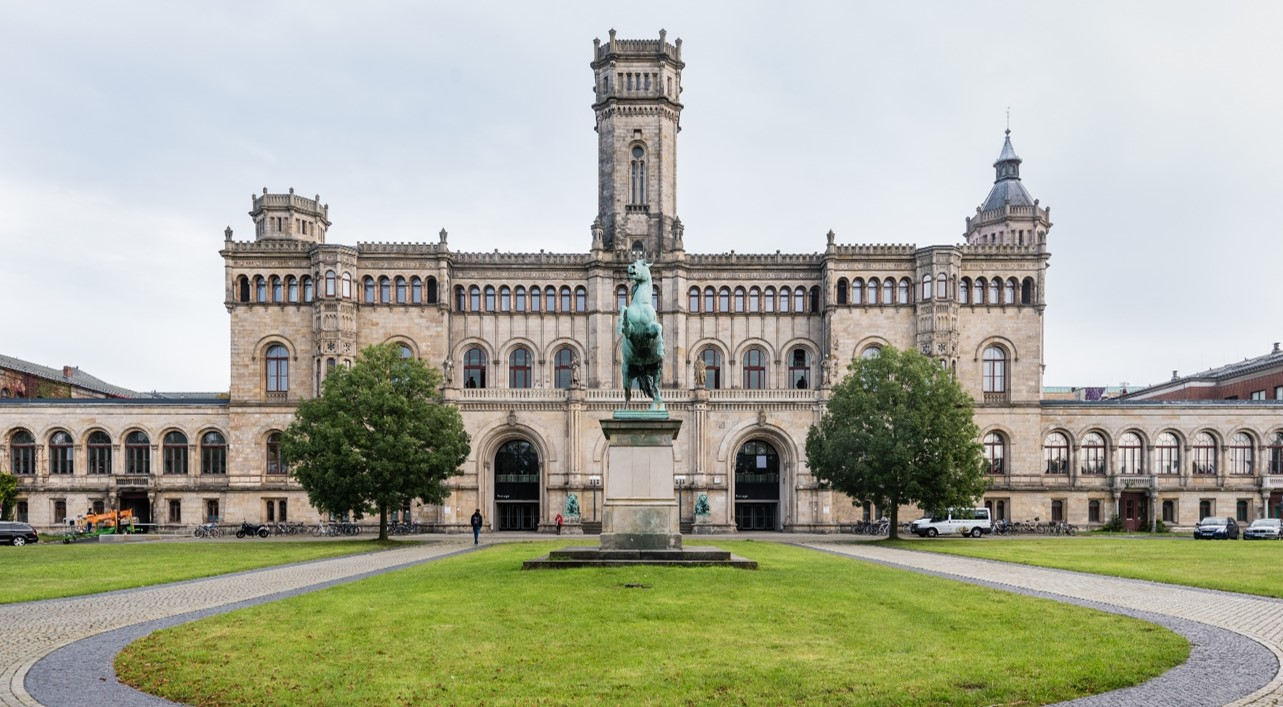
\includegraphics[width=0.65\textwidth]{figures/luh_default_presentation_title_image.jpg}}

% Title page: luhstyle
% \setbeamertemplate{title page}[luhstyle]
% % Add optional title image here
% \addtitlepageimage{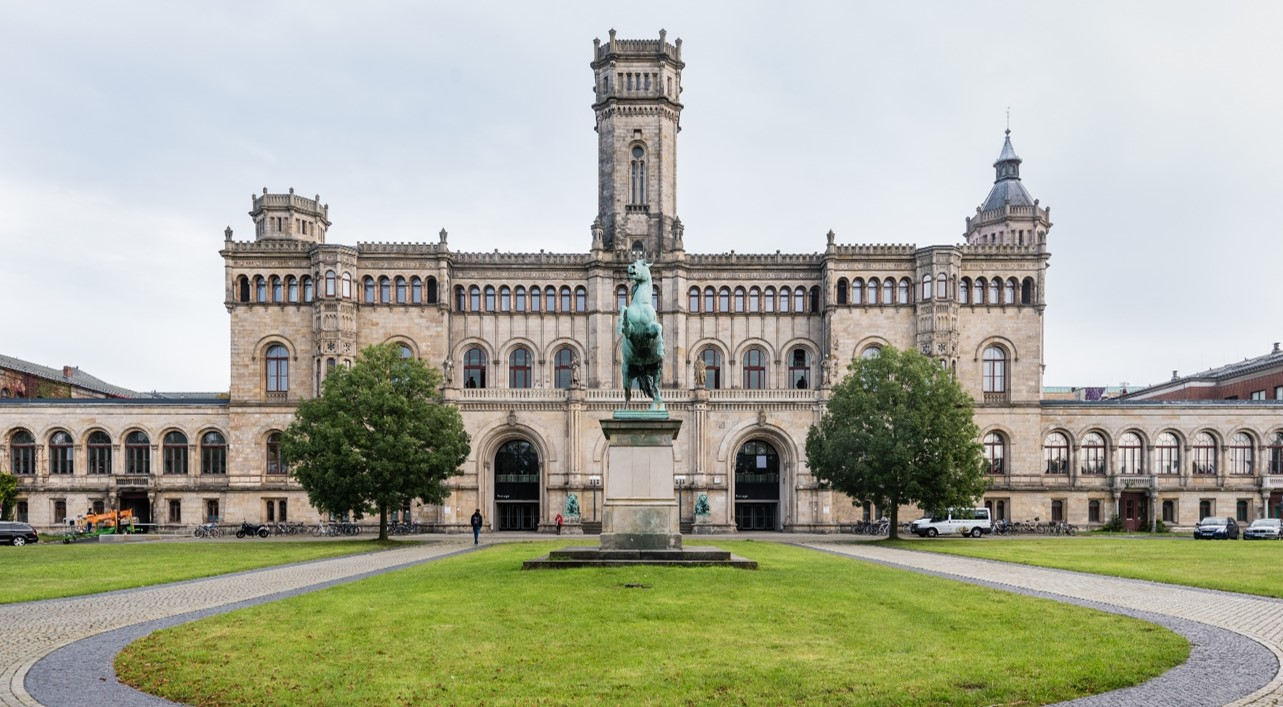
\includegraphics[width=0.75\textwidth]{figures/luh_default_presentation_title_image.jpg}}

\author[Abedjan \& Lindauer]{Ziawasch Abedjan \& Marius Lindauer\\[1em]
	
\includegraphics[height=\logoheight]{../latex_main/figures/luh_logo_rgb_0_80_155.pdf}\qquad
	
\includegraphics[height=\logoheight]{../latex_main/figures/DBIS_Kurzlogo.png}\qquad

\includegraphics[height=\logoheight]{../latex_main/figures/TNT_darkv4}\qquad

\includegraphics[height=\logoheight]{../latex_main/figures/L3S.jpg}	}
\date{Summer Term 2022; \hspace{0.5em} {
\includegraphics[height=1.5em]{../latex_main/figures/Cc-by-nc-sa_icon.svg.png}}; based on \href{https://ds100.org/fa21/}{[DS100]}
}


%%% Custom Packages
%----------------------------------------------------------------------
% Create dummy content
\usepackage{blindtext}

% Adds a frame with the current page layout. Just call \layout inside of a frame.
\usepackage{layout}


%%% Macros
%\renewcommand{\vec}[1]{\mathbf{#1}}
% \usepackage{bm}
%\let\vecb\bm

\title[Statistics]{DS: Dimension Reduction}
\subtitle{Multi-Dimensional Scaling}

\graphicspath{ {./figure/} }
%\institute{}


\begin{document}
	
	\maketitle
	
    \begin{frame}[c]{Motivation}
        
        \begin{itemize}
            \item Let's assume that we have $d$ features in our input space, but we would like to go down to $d'$ features
            \begin{itemize}
                \item $d'$ could be 2 in case we want to visualize our data
                \item Note: we only talk about $X$ and not about $y$ in any way here
            \end{itemize}
            \medskip
            \item What would be the best way to project down from $d$ features to $d'$ features?
            \item Main idea
            \begin{itemize}
                \item The information should be minimal!
                \item Information is best preserved if the distance between two points $x_i$ and $x_j$ in the $d$-dimensional space is roughly the same in the $d'$-dimensional space:
                $$ ||x_i - x_j || \approx || x'_i - x'_j || $$
                \item $||\cdot||$ can be any vector norm, e.g., Euclidean norm, but doesn't have to.
            \end{itemize}
        \end{itemize}

	\end{frame}
	
	\begin{frame}[c]{MDS Objective}
        
         $$\argmin_{x'_1, \ldots x'_M \in \mathbb{R}^{d'}} \sum_{i< j}  (||x_i - x_j || - || x'_i - x'_j ||)^2$$
        
        \begin{itemize}
            
            \item Note that $||x_i - x_j ||$ is fixed since the data is given
            \item We can only change our projected points $x'$
            \item[$\leadsto$] Depending on the vector norm and other assumptions different optimization approaches can be used to solve it
        \end{itemize}
        
	\end{frame}
	
	\begin{frame}[c]{MDS with Extensions}
        
        \begin{columns}
        
        \begin{column}{0.5\textwidth}
        
        \begin{itemize}
            \item Plot predictions in background
            \item Plot labels with different points
            \smallskip
            \item Note: 
            \begin{itemize}
                \item Categorical features can lead to separated regions
                \item axes-scales have no real meaning anymore
                \item Scale your data first if your vector does not care of same scales 
            \end{itemize}
        \end{itemize}
        
        \end{column}
        
        \begin{column}{0.5\textwidth}
        
        \begin{center}
            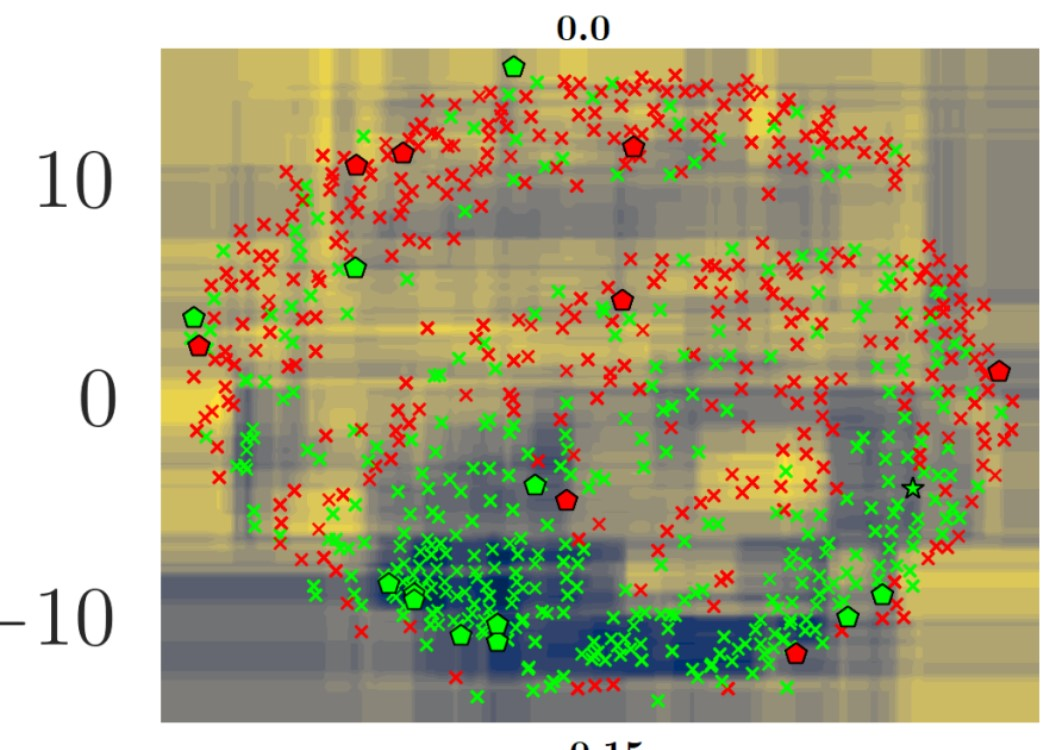
\includegraphics[width=1\textwidth]{mds1.jpg}
        \end{center}
        
        \end{column}
        
        \end{columns}
        
	\end{frame}
	
	\begin{frame}[c]{MDS with Clusters}
        
        \begin{columns}
        
        \begin{column}{0.5\textwidth}
        
        \begin{itemize}
            \item If you have dense clusters in your data, MDS will zoom in on these
            \item Could be a hint that your i.i.d. assumption is violated
        \end{itemize}
        
        \end{column}
        
        \begin{column}{0.5\textwidth}
        
        \begin{center}
            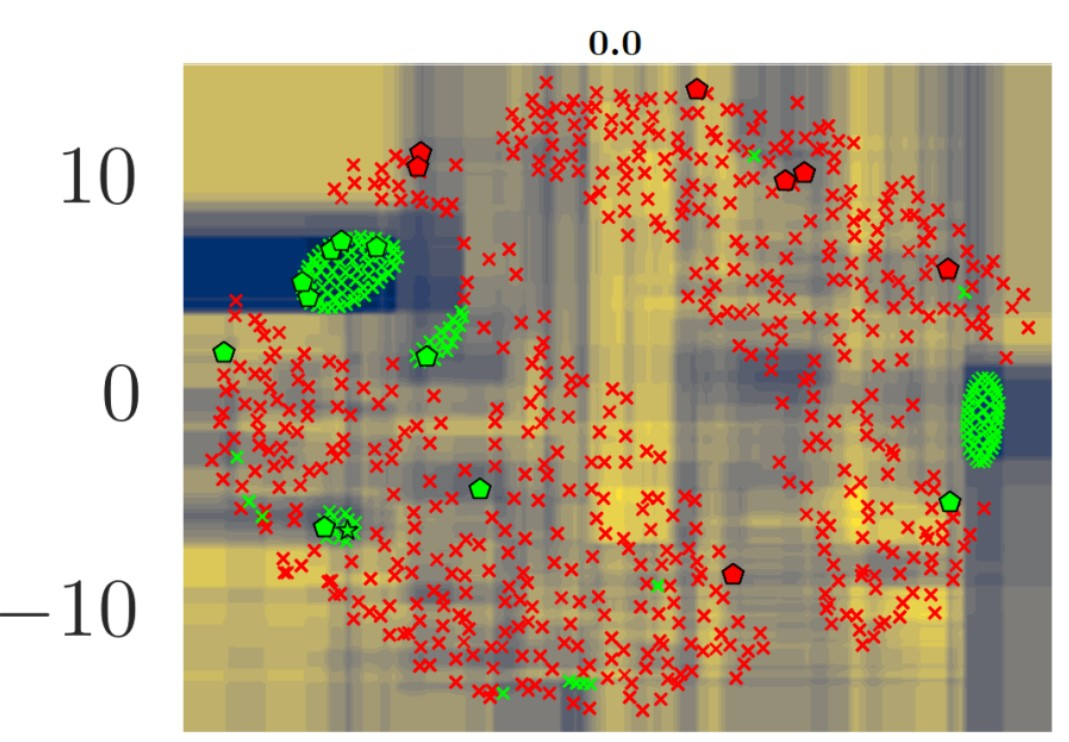
\includegraphics[width=1\textwidth]{mds2.jpg}
        \end{center}
        
        \end{column}
        
        \end{columns}
        
	\end{frame}
	
\end{document}